\documentclass[11pt,a4paper]{article}
\usepackage[ngerman]{babel}
\usepackage[T1]{fontenc}
\usepackage[utf8]{inputenc}
\usepackage[margin=2.2cm]{geometry}
\usepackage{lmodern}
\usepackage{graphicx}
\usepackage{booktabs}
\usepackage{array}
\usepackage{fancyvrb}
\usepackage{listings}
\usepackage{xcolor}
\usepackage{float}
\usepackage{hyperref}

\lstset{basicstyle=\ttfamily\footnotesize, frame=single, columns=fullflexible,
        keywordstyle=\color{blue}\bfseries, commentstyle=\color{green!50!black}}
\lstdefinelanguage{SV}{morekeywords={module,endmodule,input,output,logic,always_ff,
        begin,end,assign,if,else,posedge,negedge,or,parameter,int}, morecomment=[l]{//}}

\title{Assignment 03 -- Program Counter, Register und Speicher\\\large EIT HDL -- Doku}
\author{Lukas Wolf}
\date{\today}

\begin{document}
\maketitle

\section{Aufgabe}
Für die HACK-CPU werden sequentielle Bausteine benötigt:
\begin{itemize}
  \item \texttt{dreg}: D-Register (Breite \texttt{W}, Default 16) mit asynchronem,
        low-aktivem Reset und Übernahme bei \texttt{load \& en}.
  \item \texttt{pcount}: Program Counter (Breite \texttt{W}, Default 15) mit Reset, parallelem
        Laden (\texttt{load \& en}) und Inkrementieren (\texttt{inc \& en}).
  \item \texttt{ram16k\_verilog}: vorgegebener 16k$\times$16-Bit-Datenspeicher, der nur verifiziert wird.
\end{itemize}
Alle Takte sind 50\,MHz (\texttt{clk50m}, 20\,ns Periode), aktive Flanke ist die steigende.

\section{Implementierung}
Beide Module sind mit einem einzigen \texttt{always\_ff}-Block umgesetzt. Der Reset steht in
der Sensitivitätsliste (\texttt{negedge rst\_n}) und wirkt dadurch asynchron. Die Reihenfolge
der \texttt{if}-Zweige entspricht genau der Priorität aus der Angabe. Fehlt ein \texttt{else},
behält das Register seinen Wert.

\subsection*{D-Register}
\begin{lstlisting}[language=SV]
always_ff @(posedge clk50m or negedge rst_n) begin
    if (!rst_n)
        q <= '0;
    else if (load && en)
        q <= d;
end
\end{lstlisting}

\subsection*{Program Counter}
\begin{lstlisting}[language=SV]
always_ff @(posedge clk50m or negedge rst_n) begin
    if (!rst_n)
        cnt <= '0;
    else if (load && en)
        cnt <= cnt_in;
    else if (inc && en)
        cnt <= cnt + 1'b1;     // laeuft bei 2^W-1 auf 0 ueber
end
\end{lstlisting}

\subsection*{RAM}
Der Code aus der Angabe wurde unverändert übernommen. Geschrieben wird synchron bei
\texttt{wren = 1}, gelesen asynchron (\texttt{assign q = mem[address]}). \texttt{aclr} ist
ohne Funktion.

\section{Verifikation}
Alle drei Testbenches sind gleich aufgebaut: Die Eingänge werden bei der fallenden Flanke
angelegt, 1\,ns nach der steigenden Flanke wird der Ausgang mit dem Erwartungswert
(\texttt{tb\_exp}) verglichen. Fehler werden in \texttt{errors} gezählt, am Ende wird PASS
oder FAIL ausgegeben. Gestartet wird jeweils mit \texttt{do sim\_tb\_<name>.tcl} im
Ordner \texttt{sim}; das Skript kompiliert, simuliert und öffnet das Wave-Fenster.

Der asynchrone Reset wird geprüft, indem \texttt{rst\_n} eine Viertelperiode nach einer
Taktflanke auf 0 gezogen und 1\,ns später -- also ohne Taktflanke -- der Ausgang geprüft wird.

\subsection{D-Register (\texttt{tb\_dreg})}
Getestet: Reset (auch bei gesetztem \texttt{load \& en}), Laden von \texttt{0x0000},
\texttt{0xffff}, \texttt{0xaa55}, \texttt{0x55aa}, Halten bei \texttt{load = 0} bzw.
\texttt{en = 0} und asynchroner Reset.

\VerbatimInput[fontsize=\scriptsize, frame=single]{transcript_dreg.txt}

\begin{figure}[H]\centering
  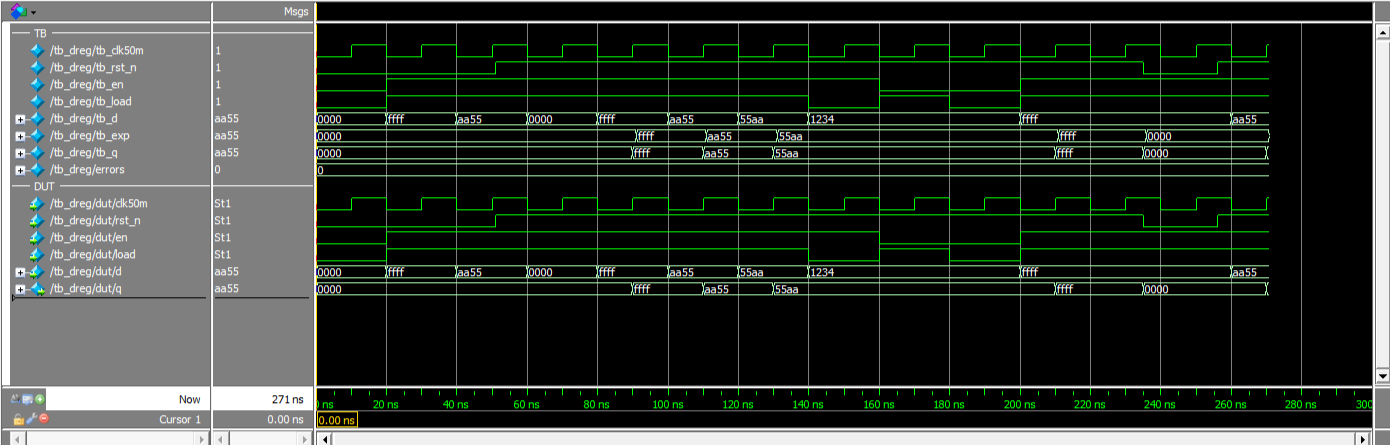
\includegraphics[width=\linewidth]{modelsim_dreg.png}
  \caption{Wave-Fenster \texttt{tb\_dreg}: \texttt{q} übernimmt \texttt{d} erst bei der
  steigenden Flanke; bei 235\,ns geht \texttt{q} sofort mit \texttt{rst\_n} auf 0.}
\end{figure}

\subsection{Program Counter (\texttt{tb\_pcount})}
Getestet: Reset, Inkrementieren, Laden, Vorrang von \texttt{load} gegenüber \texttt{inc},
Halten bei \texttt{en = 0}, Überlauf \texttt{0x7fff} $\rightarrow$ \texttt{0x0000},
16 Takte durchgehend zählen und asynchroner Reset.

\VerbatimInput[fontsize=\scriptsize, frame=single]{transcript_pcount.txt}

\begin{figure}[H]\centering
  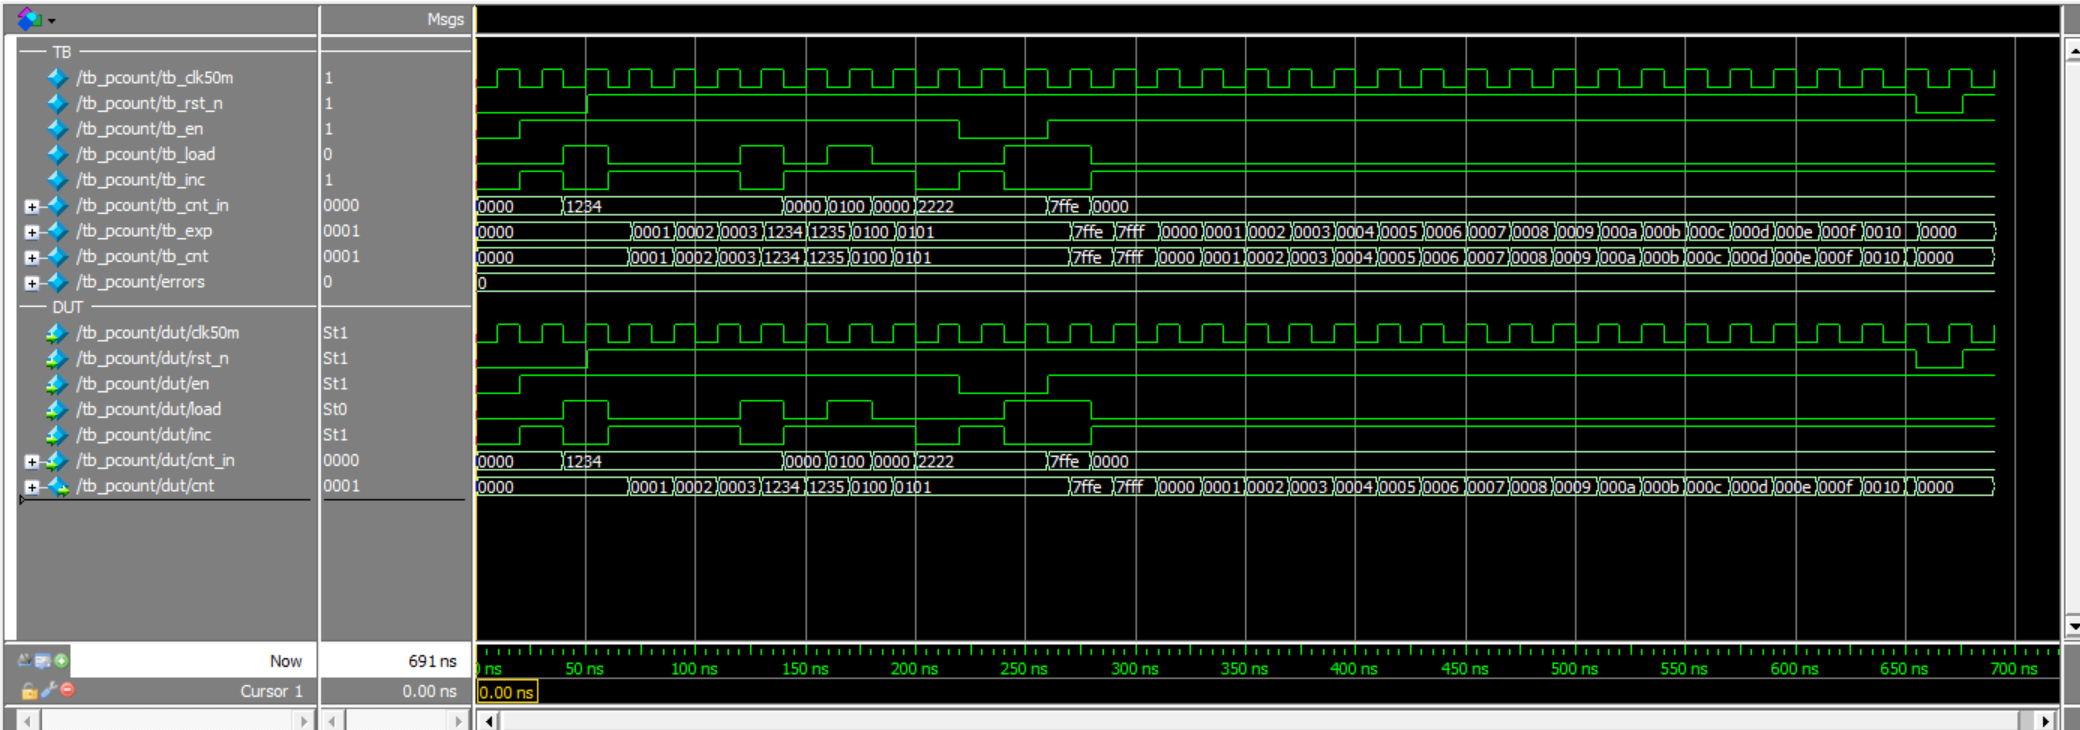
\includegraphics[width=\linewidth]{modelsim_pcount.png}
  \caption{Wave-Fenster \texttt{tb\_pcount}.}
\end{figure}

\subsection{16k-RAM (\texttt{tb\_ram16k\_verilog})}
Der gesamte Speicher (16384 Wörter) wird nacheinander mit drei Mustern beschrieben und
danach vollständig zurückgelesen und geprüft:
alle Nullen, alle Einsen (\texttt{0xffff}) und jede Zelle mit ihrer eigenen Adresse
(\texttt{mem[a] = a}). Zusätzlich wird geprüft, dass bei \texttt{wren = 0} nicht geschrieben wird.

\VerbatimInput[fontsize=\scriptsize, frame=single]{transcript_ram16k_verilog.txt}

\begin{figure}[H]\centering
  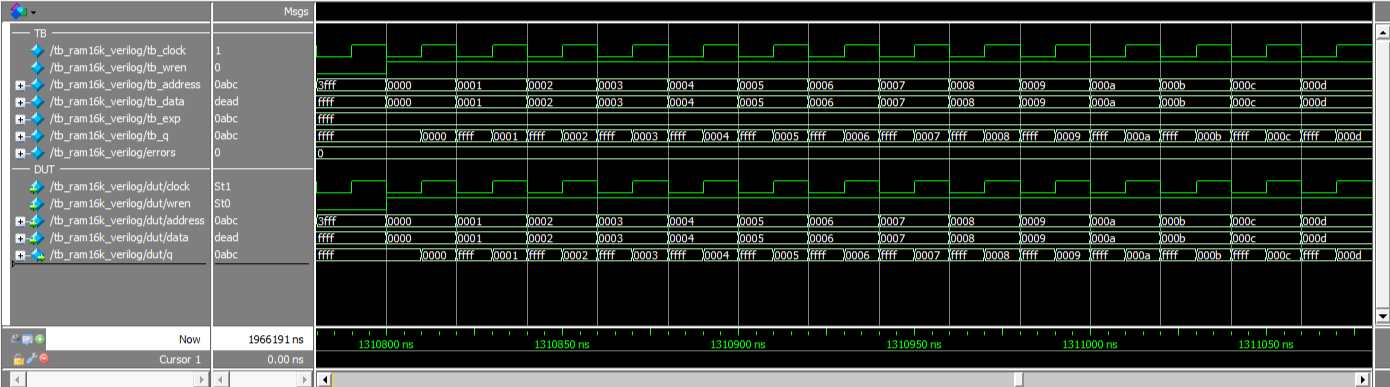
\includegraphics[width=\linewidth]{modelsim_ram16k_verilog.png}
  \caption{Wave-Fenster \texttt{tb\_ram16k\_verilog} beim Schreiben des Musters
  \glqq Wert = Adresse\grqq: \texttt{q} zeigt zuerst den alten Inhalt \texttt{0xffff}, nach der
  steigenden Flanke den neuen Wert.}
\end{figure}

\paragraph{Ergebnis} Alle drei Testbenches melden PASS, der Fehlerzähler bleibt 0. Die Module
erfüllen damit die Spezifikation.

\section{Diskussion der Implementierungsart}
\begin{tabular}{>{\raggedright}p{3.4cm}>{\raggedright}p{5.8cm}>{\raggedright\arraybackslash}p{5.8cm}}
\toprule
Methode & Vorteile & Nachteile \\ \midrule
Gatter / einzelne Flip-Flops &
Aufbau ist bis ins Detail sichtbar (wie bei nand2tetris). &
Viel Code, für Zähler mit Addierer unübersichtlich und fehleranfällig. \\[1mm]
\texttt{always\_ff} + separater \texttt{always\_comb} für Folgezustand &
Klare Trennung Logik / Speicher. &
Mehr Signale und Zeilen, bei so einfachen Modulen kein Mehrwert. \\[1mm]
\textbf{ein \texttt{always\_ff} mit \texttt{if}-Kette} (gewählt) &
Kurz, die Priorität steht direkt im Code wie in der Angabe, \texttt{W} ist parametrierbar,
Quartus erkennt Register mit Enable bzw. Zähler sofort. &
Asynchroner Reset muss beim Einsatz synchron losgelassen werden
(Reset-Synchronisierer im Toplevel). \\[1mm]
Synchroner Reset &
Keine Probleme beim Loslassen des Resets. &
Entspricht nicht der Angabe (Reset soll asynchron sein). \\
\bottomrule
\end{tabular}

\paragraph{RAM} Die Intel-RAM-Blöcke unterstützen kein gleichzeitiges Löschen aller Zellen.
Mit \texttt{aclr} müsste der Speicher aus 16k$\times$16 Flip-Flops aufgebaut werden, deshalb ist
der Reset-Zweig auskommentiert und Quartus kann den Speicher als RAM erkennen. Nachteil: Nach dem Einschalten ist der
Inhalt undefiniert (in der Simulation \texttt{X}, siehe Testbench), er muss bei Bedarf per
Software gelöscht werden.

\end{document}
